\section{Què és?}

	Anomenem software propietari a tot aquell programa publicat sota llicències
	que reserven un o tots els drets d'ús, còpia, modificació i distribució
	al fabricant qui, pagant, concedeix un ús del programa executable al titular
	de la llicència.

	Per tant, el software \emph{propietari} o \emph{privatiu} obstrueix la llibertat
	de l'usuari final, que quan ha adquirit el programa, té uns drets limitats i fortes
	obligacions, que solen incloure la impossibilitat d'adquirir i modificar el codi font del producte
	que ell mateix ha comprat, tant com la prohibició total o parcial de la redistribució del programa.
	\cite{gnucategories}

	Per a entendre millor el software propietari, posem un exemple pràctic:	en Jaume crea un programa impressionant, amb l'ajut de diferents col·laboradors (que ho fan com a hobby),
	i distribueix el programa a través d'una llicència permissiva. Amb el temps, més gent col·labora i cada vegada,
	aquest programa fet amb l'esforç de centenars de voluntaris, adquireix més importància en el món del \emph{software}.
	En Jaume, però, segueix volent mantenir la filosofia lliure del software que la comunitat ha creat, i per tant
	manté la llicència permissiva.
	
	Un dia, una companyia, agafa tot el codi d'en Jaume, el modifica lleugerament, i
	el redistribueix amb una llicència propietària. Ara, totes les millores que es podrien haver incorporat
	al codi d'en Jaume a benefici de la comunitat, estan en mans d'una gran corporació, que no les vol compartir.
	Degut a la llicència que en Jaume ha fet servir, no té dret a res, i la comunitat que ha treballat durant tot aquest temps,
	es quedarà sense les millores que la corporació ha desenvolupat, sobre la seva base.
	
	Aquesta situació es pot evitar o repetir, tot depèn de la llicència que en Jaume esculli al crear el seu següent programa.

\section{Qui el fa?}

	El principal desenvolupador de software propietari a nivell mundial és \emph{Microsoft}, encara que hi
	ha moltes més empreses que també en creen i distribueixen, com \emph{Apple, Oracle, Adobe, VMware,
	SAP, Symantec...} \cite{propietariempreses}

\section{Ús actual}

	Avui en dia molta part del software utilitzat per la majoria de població, és propietari.

	Aquesta gran extensió del seu ús és degut a l'inversió milionària al màrketing, i a
	pactes amb productors de sistemes operatius i proveïdors d'Internet, que acorden la
	prèvia instal·lació de software propietari als ordinadors. Junt amb la falta d'informació del que 
	comporta l'ús de programes propietaris, i la falta de preocupació de la integritat dels
	nostres drets virtuals, son els motius principals de l'expansió del software propietari.

	\begin{figure}[ht!]
	\centering
	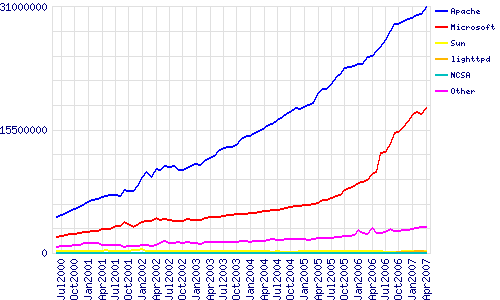
\includegraphics[width=100mm]{data/web_servers_share.png}
	\caption{Ús de software en servidors web \cite{whyfoss}}
	\label{websshare}
	\end{figure}

	\begin{figure}[h!]
	\centering
	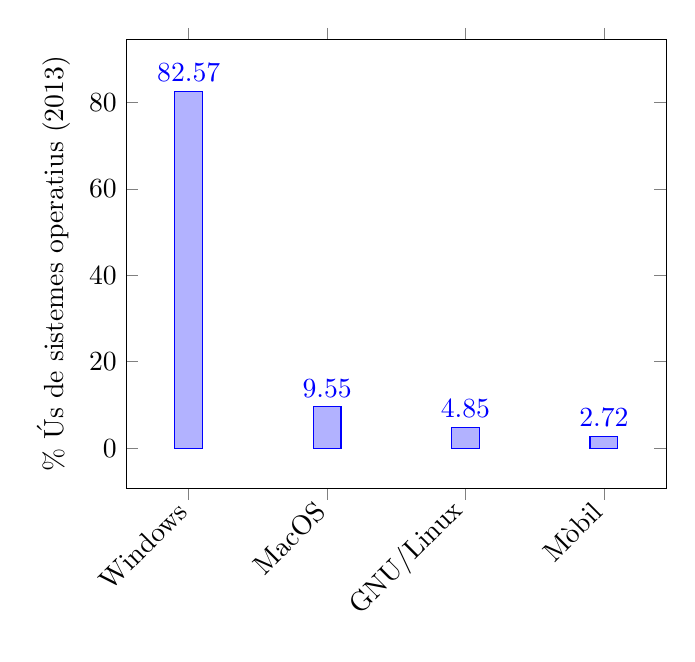
\begin{tikzpicture}
	\begin{axis}[
		ybar,
		enlargelimits=0.15,
		legend style={at={(0.5,-0.2)},
		anchor=north,legend columns=-1},
		ylabel={\% Ús de sistemes operatius (2013)},
		symbolic x coords={Windows,MacOS,GNU/Linux,Mòbil},
		xtick=data,
		nodes near coords,
		nodes near coords align={vertical},
		x tick label style={rotate=45,anchor=east},
	]
	\addplot coordinates {(Windows,82.57) (MacOS,9.55)
	(GNU/Linux,4.85) (Mòbil,2.72)};
	\end{axis}
	\end{tikzpicture}
	\caption{Ús de sistemes operatius per a particulars \cite{osstats}}
	\label{osshare}
	\end{figure}

	\begin{figure}[h!]
	\centering
	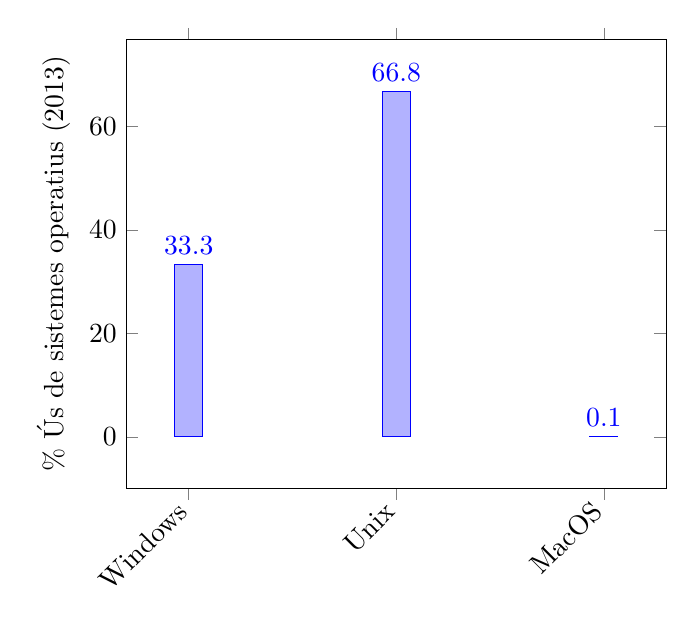
\begin{tikzpicture}
	\begin{axis}[
		ybar,
		enlargelimits=0.15,
		legend style={at={(0.5,-0.2)},
		anchor=north,legend columns=-1},
		ylabel={\% Ús de sistemes operatius (2013)},
		symbolic x coords={Windows,Unix,MacOS},
		xtick=data,
		nodes near coords,
		nodes near coords align={vertical},
		x tick label style={rotate=45,anchor=east},
	]
	\addplot coordinates {(Unix,66.8) (Windows,33.3) (MacOS,0.1)};
	\end{axis}
	\end{tikzpicture}
	\caption{Ús de sistemes operatius per a servidors \cite{ossvstats}}
	\label{ossvshare}
	\end{figure}

	El gràfic \ref{websshare} mostra la distribució (o \emph{market share}) de diferents companyies de software
	en l'àmbit dels servidors web
	\footnote{Ordinadors que funcionen el màxim de temps possible i comparteixen l'accés a una direcció web.
	Per exemple, \emph{Google} té molts servidors que permeten l'accés públic als seus serveis.}.
	\emph{Apache}\cite{apache} ha mantingut sempre la seva posició,
	seguit per \emph{Microsoft} i altres companyies. En aquest cas, el software lliure (de la mà de la
	llicència \emph{Apache 2.0}\cite{apachelicense}) és prevalent de llarg.

	El gràfic \ref{osshare} mostra el market share de \emph{sistemes operatius} que utilitzen els particulars
	(qualsevol persona). \emph{Microsoft Windows} és el guanyador indiscutible, amb \emph{MacOS} molt per darrere
	i els sistemes operatius \emph{GNU/Linux} (l'alternativa lliure) amb menys del 5\% del share.

	El gràfic \ref{ossvshare} mostra el market share de sistemes operatius que utilitzen els servidors i,
	al igual que en els programes que utilitzen els servidors, el software lliure guanya.
	
	D'aquests documents podem extreure una conclusió ben simple; la població general, no especialitzada,
	utilitza generalment software propietari (que, casualment, els hi ve pre-instal·lat als ordinadors).
	En canvi, els usuaris especialitzats (mantenidors de servidors, en aquest cas), es passen a les alternatives
	de software lliure, que amb el temps han demostrat més viabilitat i seguretat per al ús que s'els hi ha de donar.
	Per tant, el software propietari és majoritari per \emph{conveniència}, no per qualitat.


\section{Avantatges i inconvenients}

Els avantatges principals del software propietari  són ben simples; solen ser avantatges per part
de l'empresa creadora, ja que generen beneficis més elevats que el software lliure (que es sol distribuir
de forma gratuïta) \cite{gentegeek}.

Per part de l'usuari, en podem extreure alguns:

\begin{itemize}
\item \emph{Atenció al client}: molt software lliure no ofereix ni garanties, ni atenció al client 'professional'.
La major part d'empreses de software propietari es veuen obligades a oferir-ne, ja que si no, el seu producte (generalment,
que comporta un cost econòmic) perd reputació i clientela.
\item \emph{Fàcil adquisició:} avantatge per a alguns, inconvenient per a uns altres (no volen software pre-instal·lat als seus
ordinadors).
\end{itemize}

En quant a inconvenients, en podem trobar bastants:
\begin{itemize}
\item \emph{Falta de suport multi-plataforma}: molt software privatiu es centra en les plataformes principals (Windows i MacOS),
i s'oblida de les minoritàries.
\item \emph{Impossibilitat de modificació}: un programa propietari té un error amb solució simple, i tu tens coneixements de
programació? Oblida't d'arreglar-ho, hauràs d'esperar a una actualització oficial.
\item \emph{Impossibilitat de còpia}: en molts casos, si vols instal·lar un mateix software a diferents ordinadors de la teva
propietat, hauràs de comprar la mateixa llicència vàries vegades.
\item \emph{Falta de seguretat personal}: no pots saber si el software recull dades del teu ordinador, ni a qui les comparteix.
\item \emph{Dependència a l'empresa}: quan compres un programa, quedes subjugat a les decisions que l'empresa faci sobre el mateix.
\end{itemize}

\begin{figure}[ht!]
\centering
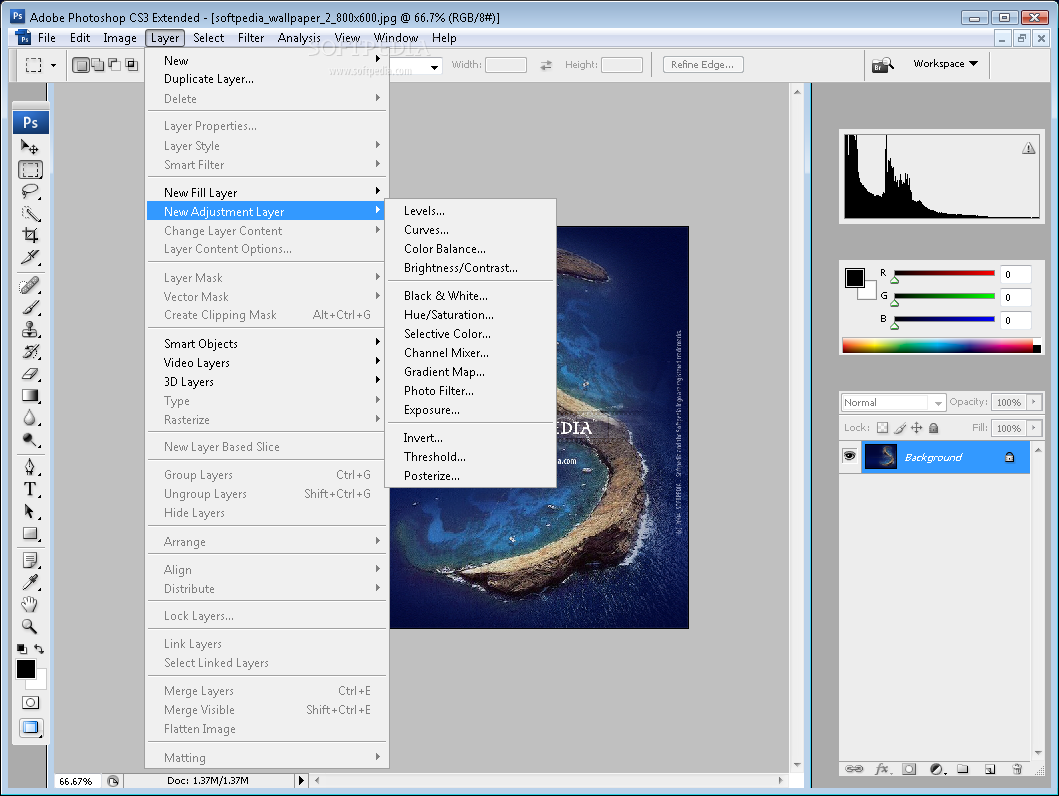
\includegraphics[height=70mm]{data/photoshop.png}
\caption{Captura del programa propietari \emph{Photoshop CS3}.}
\label{photoshop}
\end{figure}

\begin{figure}[ht!]
\centering
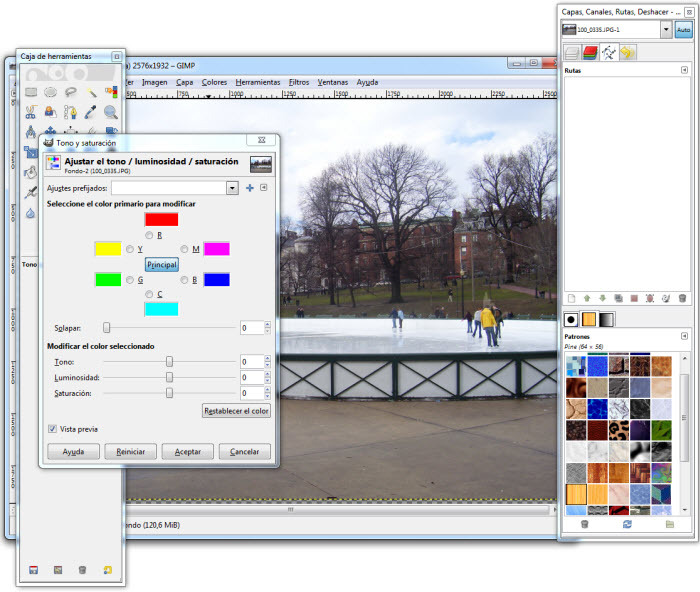
\includegraphics[height=70mm]{data/gimp.jpg}
\caption{Captura de l'alternativa lliure de Photoshop, \emph{GIMP} (GNU Image Manipulation Program)}
\label{gimp}
\end{figure}

